\chapter{Media Item Extraction}
\label{cha:media-item-extraction}

% the code below specifies where the figures are stored
\ifpdf
    \graphicspath{{5_media_item_extraction/figures/PNG/}{5_media_item_extraction/figures/PDF/}{5_media_item_extraction/figures/}}
\else
    \graphicspath{{5_media_item_extraction/figures/EPS/}{5_media_item_extraction/figures/}}
\fi

\section{Introduction}

Before the rise of social networks,
event coverage was mostly an affair of professional news agencies.
The widespread availability of mobile phones
with higher resolution cameras has transformed
citizens into witnesses who are used to comment
and share media illustrating events on social networks.
Some examples with global impact
include the shootings in
Ut{\o}ya,\footnote{\url{http://en.wikipedia.org/wiki/2011_Norway_attacks},
accessed July 15, 2013}
which first appeared on Twitter,
the capture and arrest of Muammar
Gaddafi,\footnote{\url{http://en.wikipedia.org/wiki/Death_of_Muammar_Gaddafi},
accessed July 15, 2013}
which first appeared on YouTube,
or the emergency ditching of a~plane in the Hudson
river,\footnote{\url{http://en.wikipedia.org/wiki/US_Airways_Flight_1549},
accessed July 15, 2013}
which first appeared on Twitpic.
Some news
communities\footnote{\url{http://www.citizenside.com/},
accessed July 15, 2013}
have even specialized in aggregating and brokering
such user-generated content.
Events, such as sports matches or concerts are 
largely illustrated by social media,
albeit distributed over many social networks.

In this chapter, we tackle the challenge of reconciling
social media data that illustrates known events,
but that is spread over various social networks,
all with the objective of creating visual event summaries.
We propose a~social-network-agnostic
approach for the extraction of photos and videos covering events.
We want to emphasize that in this chapter we do \emph{not}
put the focus on event detection (we have done that in \autoref{cha:eventdetection}). 
The events we are dealing with in this chapter
were known beforehand and we use specific
human-chosen search terms to find illustrating media.

We first recall the definitions previously made in
\autoref{sec:definition} and add formal definitions
of the terms \emph{event},
\emph{media item extraction},
\emph{Application Programming Interface},
and \emph{Web scraping}.

\begin{description}
  \item[Social Network:]
       A~social network is an online service or media platform
       that focuses on building and reflecting
       relationships among people
       who share interests and/or activities.
  \item[Media Item:]
       A~media item is defined as
       a~photo\footnote{We choose the term \emph{photo}
       over the term \emph{image} as 
       Facebook, Twitter, and \googleplus use it}
       or video file that is publicly shared or published
       on at least one social network.
  \item[Micropost:]
       A~micropost is defined as a~textual status message
       that can optionally be accompanied by a~media item.
  \item[Event:]
       An event is defined as a~phenomenon that has happened
       or that is scheduled to happen.
       It is an observable occurrence grouping persons,
       places, times, and activities while being often
       documented by people through different media~%
       \cite{liu2011events}.
  \item[Media Item Extraction:]
       The process of leveraging search functionalities of
       social networks to find references to media items,
       which allows for storing those media items in binary form.       
  \item[Application Programming Interface (API):]
       An API is a~programmatic specification intended to be used
       as an interface by software components on client and server
       to communicate with each other.
  \item[Web scraping]
       The term Web scraping means the process of
       automatedly extracting information from Web pages.
       Web scraping involves practical solutions based on
       existing technologies that are often entirely \emph{ad hoc}.
       Examples of such technologies are regular expressions,
       Document Object Model (DOM)
       parsing~\cite{lehors2004dom},
       or CSS selectors~\cite{hunt2012cssselectors}.
       The difference between \emph{Web scraping}
       and the related concept of \emph{screen scraping}
       is that screen scraping relies on the visual layout of a~Web page,
       while Web scraping relies on the textual
       and/or hierarchical structure of Web pages.
\end{description}


\section{Related Work}

Related work covers research
that aims to collect, align, and organize media
for trends or events.
Liu \emph{et~al.}\ combine semantic inferencing and visual analysis
to automatically find media to illustrate
events~\cite{liu2011events}.
They interlink large datasets of event metadata
and media with the Linking Open Data
Cloud~\cite{bizer2011statelodcloud,cyganiak2011lodcloud}.
In~\cite{liu2011socialmedia}, they show how visual summaries
of past events providing viewers with a~more compelling feeling
of the event's atmosphere can be created
based on a~method to automatically detect and identify events
from social media sharing websites.
Approaches to alignment use visual, temporal,
and spacial similarity measures to map multiple photo streams of
the same events~\cite{yang2011photostream}.
Other ways to collect and order media from social networks use
media-driven metadata such as geospatial
information~\cite{crandall2009mappingphotos}.
Becker \emph{et~al.}\ show in~\cite{becker2010eventidentification}
how to exploit the rich context associated with social media
content, including user-provided annotations
and automatically generated information.
Using this rich context, they define document similarity metrics
to enable online clustering of media to events.
In~\cite{becker2012plannedevents}, the same authors develop 
recall-oriented query formulation strategies
based on noisy event metadata
from event aggregation platforms.

\section{Social Networks and Media Items}                                    \label{sec:social-networks}

Most social networks offer a~search functionality that allows for
content to be retrieved based on search terms,
with or without more advanced search operators
such as exclusion, inclusion, phrase search, \emph{etc.}
Each social network has special constraints
regarding the supported search operators or filtering options.

Social networks are often perceived as
\emph{walled gardens}~\cite{simonds2008walledgarden}
due to the full control of the network operator
over content and media on the social network in question,
oftentimes accessible exclusively by social network members.
This network lock-in effect was excellently illustrated
by David Simonds in a~cartoon that first appeared
in the English-language weekly news and
international affairs publication \emph{The Economist},
reproduced in \autoref{fig:walled-gardens}.
While some social networks (\emph{e.g.}, Twitter)
have full read and write access via specified APIs,
other social networks (\emph{e.g.}, \googleplus)
currently only have read API access.
In some cases, however, API access is limited,
so that not all desired pieces of information is exposed
(\emph{e.g.}, view counts with Img.ly),
which forces people interested in that data
to fall back to Web scraping.
It is to be noted that Web scraping \emph{per~se}
is not an illegal practice, as only public information is being accessed,
comparable to the level of access that common Web search engines have.

\begin{figure}[!ht]
  \centering
  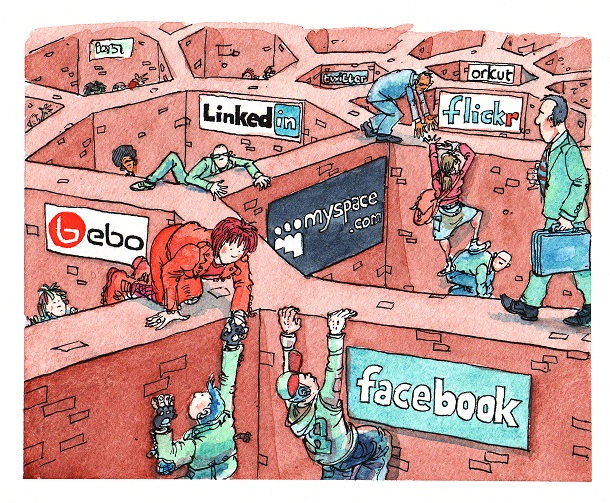
\includegraphics[width=0.7\linewidth,
    trim=16px 17px 12px 15px,clip]{davidsimonds.jpg}
  \caption[Social networks as walled
    gardens illustrated by David Simonds]
    {Social networks as walled gardens illustrated by David Simonds}
  \label{fig:walled-gardens}
\end{figure}

\section{Media Extractor}
\label{sec:media-extractor}

In this section, we first introduce a~common data format
that we have developed as an abstraction layer on top of the native
data formats used by the considered social networks.
We then explain the architecture
of different kinds of media item extractors.
Finally, we describe the various processing steps
that we apply to each collected media item.

\subsection{Abstraction Layer Data Format}
\label{sec:data-format}

Each social network uses a~different data representation schema.
While all social networks with API access are
JSON-based~\cite{crockford2006json}, the differences in both 
supported social network features and media item support level,
outlined in detail in
\autoref{sec:description-of-popular-social-networks} and
\autoref{sec:classification-of-social-networks},
are also reflected in the returned JSON data.
We therefore propose a~common abstraction layer 
on top of the native data formats of all considered social networks.
This abstraction layer is outlined in \autoref{tab:platforms}
and allows us to gain
an agnostic view on the underlying social networks.
It's in the nature of any abstraction
that it can only represent the
greatest common divisor of all social networks.
We explain the abstraction layer in the following
with the help of a~concrete example,
stemming from a~query to the media extractor
that will be explained in more detail
in the upcoming \autoref{sec:media-item-extractors}.
The media extractor was used to query for media items
that match the search term \emph{hamburg}.
\autoref{code:facebook} shows sample output of the media extractor
for a~Facebook post, which was processed
with named entity extraction and disambiguation 
as detailed in \autoref{cha:micropost-annotation}.
Below, we explain the data format of our media extractor.

\begin{description}
  \item[\texttt{mediaUrl}] Deep link to a~media item
  \item[\texttt{posterUrl}] Deep link to a~thumbnail for photos
    or still frame for videos
  \item[\texttt{micropostUrl}] Deep link to the micropost on
    the social network
  \item[\texttt{micropost}] Container for a~micropost
  \begin{description}
    \item[\texttt{html}] Text of the micropost,
      possibly with HTML      markup
    \item[\texttt{plainText}] Text of the micropost with
      potential HTML markup removed
    \item[\texttt{entities}] Extracted and disambiguated
      named entities from the micropost text
  \end{description}      
  \item[\texttt{userProfileUrl}] Deep link to the user's
    profile on the social network
  \item[\texttt{type}] Type of the media item,
    can be \texttt{photo} or \texttt{video}
  \item[\texttt{timestamp}] Number of milliseconds between
    1 January 1970 00:00:00 UTC and the moment
    when the micropost was published
  \item[\texttt{publicationDate}] Date in ISO 8601
    format (YYYY-MM-DDTHH:MM:SSZ) when the micropost was published
  \item[\texttt{socialInteractions}] Container for social
    interactions
  \begin{description}  
  \item[\texttt{likes}] Number of times a~micropost was liked, or
    \texttt{unknown}
  \item[\texttt{shares}] Number of times a~micropost was shared, or
    \texttt{unknown}
  \item[\texttt{comments}] Number of comments a~micropost
    received, or \texttt{unknown}
  \item[\texttt{views}] Number of views a~micropost reached, or
    \texttt{unknown}
  \end{description}    
\end{description}

\begin{lstlisting}[caption={[Sample output of the media extractor]{Sample output of the media extractor
  showing a~Facebook post processed with named entity extraction
  and disambiguation (slightly shortened for legibility)}},
  label={code:facebook}]
{
  "mediaUrl": "http://video.ak.fbcdn.net/...",
  "posterUrl": "http://external.ak.fbcdn.net/...",
  "micropostUrl": "https://www.facebook.com/permalink.php?story_fbid=
    231781590231029&id=1254772464",
  "micropost": {
    "html": "Videoed between Hamburg and Snyder. Thought I would share.",
    "plainText": "Videoed between Hamburg and Snyder. Thought I would share.",
    "entities": [
      [
        {
          "name": "Hamburg",
          "relevance": 0.82274,
          "uri": "http://dbpedia.org/resource/Hamburg"
        },
        {
          "name": "Snyder",
          "relevance": 0.857,
          "uri": "http://dbpedia.org/resource/Snyder,_Texas"
        }
      ]
    ]
  },
  "userProfileUrl": "https://www.facebook.com/profile.php?id=1254772464",
  "type": "video",
  "timestamp": 1326371479000,
  "publicationDate": "2012-01-12T12:31:19Z",
  "socialInteractions": {
    "likes": 0,
    "shares": 0,
    "comments": 3,
    "views": null
  }
}
\end{lstlisting}

\subsection{Media Item Extractors}
\label{sec:media-item-extractors}

We have developed a~combined media extractor composed of
separate media item extractors for the seven social networks
\googleplus, Myspace, Facebook, Twitter, Instagram, YouTube,
and Flickr, with additional support for the media sharing
platforms Img.ly, Imgur, Lockerz,\footnote{Dysfunctional since April 2013 when the service shut down its API access} Yfrog, MobyPicture, and Twitpic.
The media extractor takes as input a~search term that is relevant
to a~known event, \emph{e.g.}, the term \emph{boston celtics}
for a~recent match of the Basketball team Boston Celtics.
This search term gets forwarded to the search APIs
of all social networks in parallel.
Each social network has a~30 seconds timeout window
to deliver its results.
When the timeout is reached
or when all social networks have responded,
the available results are aligned according to the data format
defined in \autoref{sec:data-format}.
Media items and the relevant metadata like view count, comments,
\emph{etc.}\ are retrieved either directly or via Web scraping.
For some social networks, \emph{e.g.}, Img.ly,
a~combination of Web scraping and API access is required
since the API does not return all necessary fields
of our data format.
While we could default to Web scraping
to obtain all relevant data,
it is more robust to use API access wherever possible
and only fall back to the more brittle Web scraping
for the parts not covered by API access.

\paragraph{Special Role of Twitter:}

Twitter (\autoref{sec:twitter})
plays a~special role, as it can be used as
a third-order support social network,
as was detailed previously in \autoref{sec:classification-of-social-networks}.
This means that the micropost text is located on Twitter,
but the referenced media items are located
on third-party media platforms.
Due to the length limitation for tweets of 140 characters,
short URLs are used on the service.
We search for the search term in question (\emph{e.g.},
following up from the example before, \emph{boston celtics}),
but combine it with the short URL domain parts of
the media platforms.
For example, the short domain URL of the social network Flickr 
(\autoref{sec:flickr})
is \url{flic.kr}, where the long domain URL is \url{flicker.com}.
The short domain URL of Instagram 
(\autoref{sec:instagram}) is \url{instagr.am},
where the long domain URL is \url{instagram.com}, \emph{etc.}
We have created a~list of all known short domain URLs for the 
considered media platforms so that the complete search query
for Twitter is the actual search term,
combined with this list of short domain URLs:

\emph{boston celtics AND (flic.kr OR instagr.am OR ...)}

\noindent The complete data flow is illustrated in the
architectural diagram in \autoref{fig:architecture}.
As a~side note, Twitter on its website now has its own
media extractor based on Twitter Cards~\cite{wang2012twitter}
with support for some of of the media platforms,
however, our own media extractor goes beyond Twitter's offer,
especially since Facebook-owned Instagram's latest break-up with
Twitter.\footnote{\url{http://techcrunch.com/2012/12/05/kevin-systrom-on-pulling-twitter-cards-integration-we-want-images-viewed-on-instagram-com/}, accessed July 15, 2013}

\begin{figure}
  \centering
  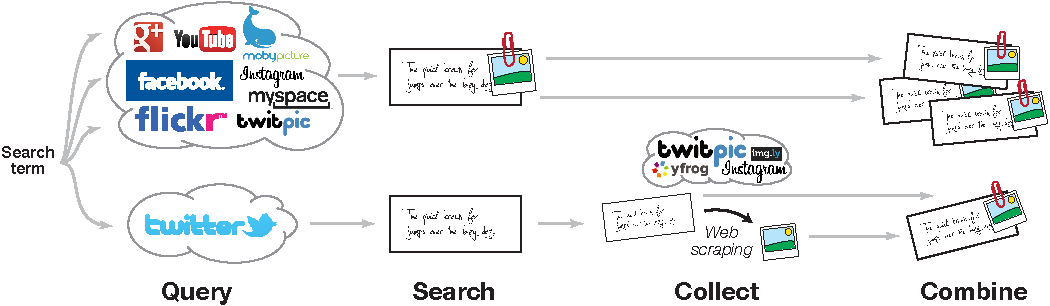
\includegraphics[width=1.0\linewidth]{architecture.pdf}
  \caption[Overview of the media extractor]
    {Overview of the media extractor:
    hybrid approach to the media item extraction task using
    a~combination of API access and Web scraping}
  \label{fig:architecture}
\end{figure}

\section{Evaluation}

We have run experiments in the time period of January 10 to 19, 2012,
during which we have randomly selected nine events
that received broad social media coverage.
For these events, we have collected media items and microposts
using our media extractor.
In the following, we will provide a~short summary of the nine selected events
in order to give the reader the necessary background knowledge.

\begin{description}
  \item[Assad Speech]
       On January 10, 2012, Syrian President Bashar al-Assad
       delivered a~televised talk defending his
       government's actions and motivations, despite world
       pressure on his government for its 10-month
       crackdown on
       protesters.\footnote{\url{http://www.cnn.com/2012/01/10/world/meast/syria-unrest/},
       accessed July 15, 2013}
  \item[CES Las Vegas]
       The International Consumer Electronics Show (CES) is
       a~major technology-related trade show held each January
       in the Las Vegas Convention Center. Not open to the public,
       the Consumer Electronics Association-sponsored show
       typically hosts previews of products and new product
       announcements.
       CES Las Vegas took place from January 11 to 13,
       2012.\footnote{\url{http://www.cesweb.org/},
       accessed July 15, 2013}\\
       \textbf{Cut the Rope Launch:}
       On January 10, 2012 during Microsoft's keynote at CES, the
       HTML5 version of the popular mobile game \textit{Cut the
       Rope} was announced. This is a~sub-event of CES Las
       Vegas.\footnote{\url{http://ces.cnet.com/8301-33377_1-57356403/},
       accessed July 15, 2013}\\       
       \textbf{Ubuntu TV Launch:}
       Ubuntu TV by Canonical, based on the user interface Unity,
       is a~variant of the Ubuntu operating system, designed to be
       a~Linux distribution specially adapted for embedded systems
       in televisions. It was announced by Canonical on January
       10, 2012, at
       CES.\footnote{\url{http://www.theverge.com/2012/1/9/2695387/ubuntu-tv-video-hands-on},
       accessed July 15, 2013}       
  \item[Costa Concordia Disaster]
       The Costa Concordia is an Italian cruise ship that hit
       a~reef and partially sank on January 13, 2012 off the
       Italian coast. The vessel ran aground at Isola del Giglio,
       Tuscany, resulting in the evacuation of 4,211
       people.\footnote{\url{http://en.wikipedia.org/wiki/Costa_Concordia_disaster},
       accessed July 15, 2013}
  \item[Dixville Notch]
       Dixville Notch is an unincorporated village in Dixville
       township of Coos County, New Hampshire, USA, best known in
       connection with its longstanding middle-of-the-night vote in
       the U.S. presidential election. In a~tradition that started
       in the 1960 election, all the eligible voters in Dixville
       Notch gather at midnight in the ballroom of The Balsams.
       This year, on January 10, 2012, the voters cast their
       ballots and the polls officially closed one minute
       later.\footnote{\url{http://www.washingtonpost.com/2012/01/09/gIQANslKnP_story.html},
       accessed July 15, 2013}
  \item[Free Mobile Launch]
       Free Mobile is a~French mobile broadband company, part of
       the Iliad group. On January 10, 2012, a~long-awaited mobile
       phone package for \EUR{19.99} with calls included to 40
       countries, texts, multimedia messages and Internet was
       announced by the Iliad group's Chief Strategy Officer
       Xavier
       Niel.\footnote{\url{http://www.nytimes.com/2012/01/11/technology/iliad-takes-aim-at-top-mobile-operators-in-france.html},
       accessed July 15, 2013}
  \item[Blackout SOPA]
       The Stop Online Piracy Act (SOPA) is a~bill of the United
       States proposed in 2011 to fight online trafficking in
       copyrighted intellectual property and counterfeit goods.
       On January 18, the English Wikipedia, and several
       other Internet companies coordinated a~service blackout
       to protest SOPA and its sister bill, the Protect IP Act
       (PIPA).
       Other companies, including Google, posted links and
       photos in an effort to raise
       awareness.\footnote{\url{http://sopablackout.org/learnmore/},
       accessed July 15, 2013}
  \item[Christian Wulff Case]
       Since December 2011, former German President Christian
       Wulff faces controversy over discrepancies in statements
       about a~loan while being governor of Lower Saxony.
       It was revealed that he had applied pressure
       on Springer Press to delay revelations on the issue until
       he was back from a~visit abroad. When Wulff found out that
       a~tabloid was going to break the story, he left a~message
       on their voice mail in which he threatened to take legal
       action.\footnote{\url{http://www.spiegel.de/international/germany/0,1518,804631,00.html},
       accessed July 15, 2013}
\end{description}

\subsection{Dataset}
Our data set contained 448 photos with an average file size of
$\sim$0.7MB and 143 videos.
Some videos are no longer available due to either
account termination or video takedown by the user
(Assad, Dixville).
\autoref{tab:number-media} shows the total
numbers of retrieved photos and videos of the media extractor.
Table cell values marked with $n+$ signify that there were more 
results, but that only $n$ results were considered. 
We have calculated the precisions for each event for both video 
and photo separately; the overall photo precision was $0.73$,
and the overall video precision was $0.54$.
We note that these values were calculated \emph{before}
any pruning step, \emph{i.e.}, before taking into account
the additional textual information from microposts like
potential extracted named entities.
The dataset is very diverse with respect to photo quality,
photo format, and naturally, content.
It ranges from entirely sharp screenshots
in all sorts of formats (\emph{e.g.},
screenshots of the Google homepage for the Blackout SOPA event
to screenshots of a~wide banner advertisement),
over to blurry cell phone photos in standard photo formats
(\emph{e.g.}, photos of the stage
for the Free Mobile Launch event).
\autoref{fig:sequences} shows sample photos for
some of the considered nine events.
We have observed that more than one search session
with different combinations of search terms~%
\cite{becker2010eventidentification,becker2012plannedevents}
is necessary in order to obtain a~satisfactory recall.
Query strategies developed by Becker~\cite{becker2012plannedevents}
that combine different combinations of event title,
event venue, and event city work consistently well.

\begin{sidewaystable}[!ht]
  \centering
  \footnotesize
  \begin{tabular}{|l|c|c|c|c|c|c|c|c|c|c|c|c|c|c|c|c|c|c|}
    \hline
    \multicolumn{1}{|c|}{\textbf{Social}} & \multicolumn{2}{c|}{\textbf{Assad}} & \multicolumn{2}{c|}{\textbf{CES}} &
    \multicolumn{2}{c|}{\textbf{Concordia}} & \multicolumn{2}{c|}{\textbf{Dixville}} & \multicolumn{2}{c|}{\textbf{Free}} &
    \multicolumn{2}{c|}{\textbf{Ropes}} & \multicolumn{2}{c|}{\textbf{SOPA}} & \multicolumn{2}{c|}{\textbf{Ubuntu}} &
    \multicolumn{2}{c|}{\textbf{Wulff}} \\
    \cline{2-19}
    \multicolumn{1}{|c|}{\textbf{Network}} & \textbf{P} & \textbf{V} & \textbf{P} & \textbf{V} & \textbf{P} & \textbf{V} &
    \textbf{P} & \textbf{V} & \textbf{P} & \textbf{V} & \textbf{P} & \textbf{V} & \textbf{P} & \textbf{V} & \textbf{P} &
    \textbf{V} & \textbf{P} & \textbf{V} \\
    \hline
    \textbf{\googleplus} & 3 & 2 & 5 & 3 & 15 & 1 & 4 & 1 & 6 & 0 & 5 & 1 & 5 & 0 & 6 & 1 & 7 & 0\\
    \textbf{Myspace} & 0 & 0 & 0 & 0 & 10+ & 0 & 9 & 0 & 1 & 0 & 6 & 0 & 0 & 0 & 0 & 0 & 8 & 0\\
    \textbf{Facebook} & 0 & 0 & 0 & 1 & 0 & 1 & 0 & 0 & 0 & 0 & 0 & 0 & 0 & 2 & 0 & 0 & 0 & 0\\
    \textbf{Twitter} & 2 & 0 & 2 & 0 & 3 & 0 & 3 & 0 & 2 & 0 & 4 & 0 & 5 & 0 & 0 & 0 & 2 & 0\\
    \textbf{Instagram} & 0 & 0 & 20+ & 0 & 20+ & 0 & 0 & 0 & 20+ & 0 & 20+ & 0 & 20+ & 0 & 0 & 0 & 2 & 0\\
    \textbf{YouTube} & 0 & 10+ & 0 & 10+ & 0 & 10+ & 0 & 3 & 0 & 10+ & 0 & 10+ & 0 & 10+ & 0 & 10+ & 0 & 10+\\
    \textbf{Flickr} & 10+ & 0 & 10+ & 6 & 10+ & 10+ & 10+ & 10+ & 10+ & 0 & 10+ & 10+ & 10+ & 0 & 10+ & 9 & 10+ & 2\\
    \textbf{MobyPic} & 0 & 0 & 1 & 0 & 4 & 0 & 0 & 0 & 2 & 0 & 20+ & 0 & 1 & 0 & 2 & 0 & 3 & 0\\
    \textbf{Twitpic} & 0 & 0 & 20+ & 0 & 18 & 0 & 1 & 0 & 20+ & 0 & 20+ & 0 & 19 & 0 & 2 & 0 & 20+ & 0\\
    \hline
    \textbf{Total} & 15 & 12 & 58 & 20 & 80 & 22 & 27 & 14 & 61 & 10 & 85 & 21 & 60 & 12 & 20 & 20 & 52 & 12\\
    \hline
    \textbf{Relevant} & 12 & 7 & 39 & 18 & 61 & 15 & 8 & 2 & 46 & 4 & 76 & 14 & 43 & 5 & 18 & 13 & 39 & 7\\    
    \hline
    \hline    
    \textbf{Precision} & .80 & .58 & .67 & .90 & .76 & .55 & .30 & .14 & .75 & .40 & .89 & .67 & .71 & .42 & .90 & .65 & .75 & .58\\
    \hline  
  \end{tabular}
  \caption[Number of photos and videos collected for nine events]{Number of photos and videos collected for nine events happening between January 10--19, 2012 grouped by social networks, separated in photo (P) and video (V) results. Overall \textbf{photo precision: 0.73}. Overall \textbf{video precision: 0.54}. Note that this is before post-processing. \todo{Check final orientation}}
  \label{tab:number-media}
\end{sidewaystable}

\begin{figure*}
\begin{tabular}{p{\textwidth}}
\eventtitle{Blackout SOPA}
\begin{thumbsequence}
		
\includegraphics[height=\thumbheight]{sopa/looseduplicate1.jpg}
		
\includegraphics[height=\thumbheight]{sopa/looseduplicate2.jpg}
		
\includegraphics[height=\thumbheight]{sopa/looseduplicate3.jpg}
		
\includegraphics[height=\thumbheight]{sopa/looseduplicate4.jpg}
		
\includegraphics[height=\thumbheight]{sopa/looseduplicate5.jpg}
		
\includegraphics[height=\thumbheight]{sopa/looseduplicate6.jpg}
	\end{thumbsequence}
	\begin{thumbsequence}
		
\includegraphics[height=\thumbheight]{sopa/looseduplicate7.png}
		
\includegraphics[height=\thumbheight]{sopa/looseduplicate8.jpg}
	\end{thumbsequence}
	\newstrip
	\begin{thumbsequence}
		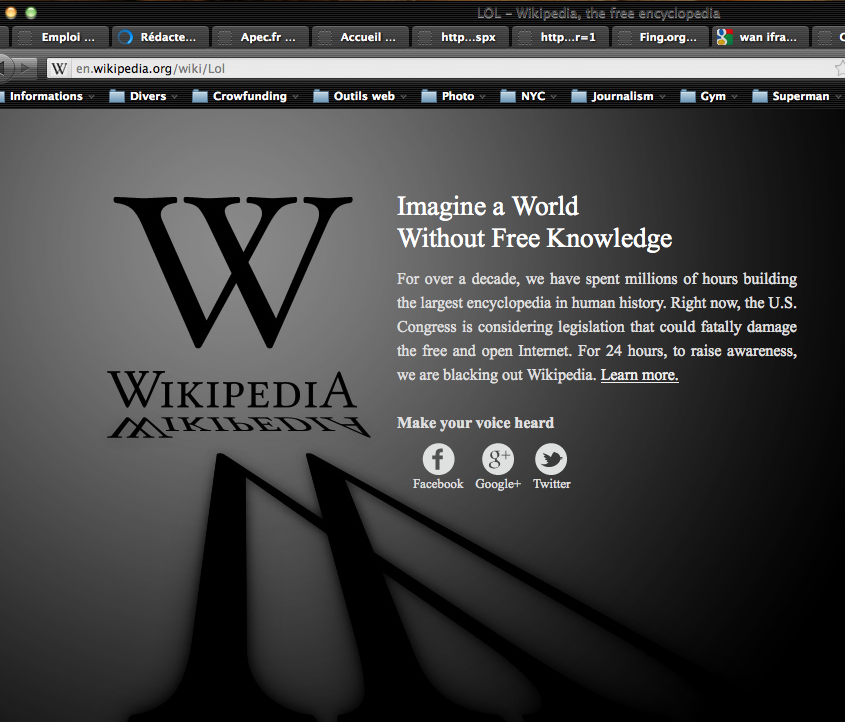
\includegraphics[height=\thumbheight]{sopa/looseduplicate9.png}
		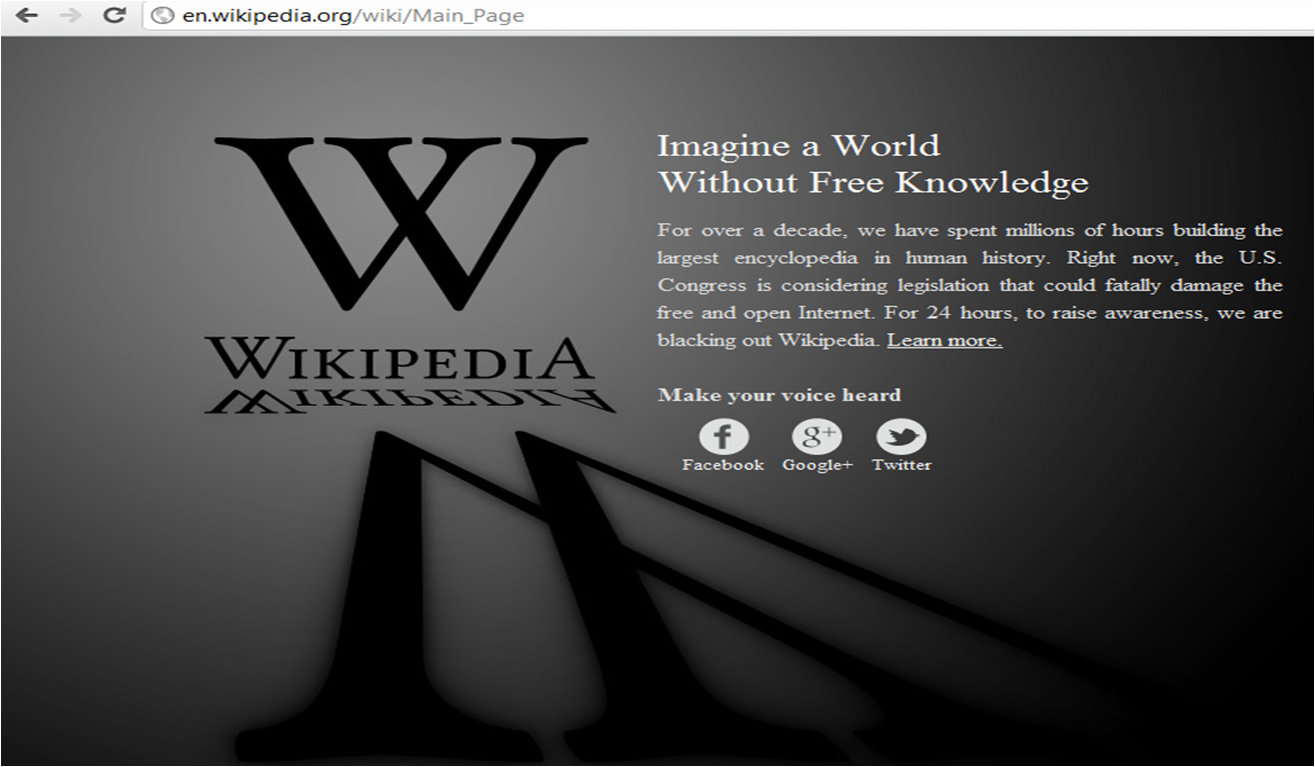
\includegraphics[height=\thumbheight]{sopa/looseduplicate10.png}
		
\includegraphics[height=\thumbheight]{sopa/looseduplicate11.jpg}
		
\includegraphics[height=\thumbheight]{sopa/looseduplicate12.jpg}
	\end{thumbsequence}
	\begin{thumbsequence}
		\setlength\fboxsep{0pt}
		\setlength\fboxrule{0.1mm}
		\fbox{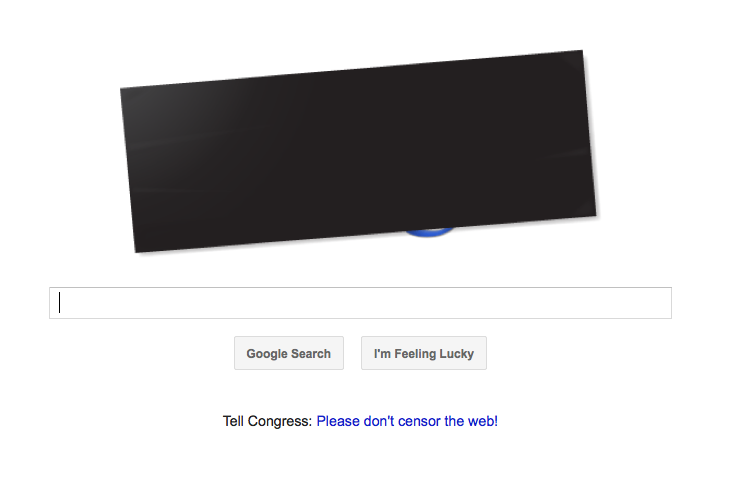
\includegraphics[height=\thumbheight]{sopa/looseduplicate13.png}}
		\fbox{
\includegraphics[height=\thumbheight]{sopa/looseduplicate14.jpg}}
\end{thumbsequence}
\end{tabular}
	
\begin{tabular}{p{\textwidth}}
\eventtitle{Christian Wulff Case}
	\begin{thumbsequence}
		\doublebox{
\includegraphics[height=\thumbheight]{wulff/exactduplicate1.jpg}}
		\doublebox{
\includegraphics[height=\thumbheight]{wulff/exactduplicate2.jpg}}
	\end{thumbsequence}
	\begin{thumbsequence}
		\doublebox{
\includegraphics[height=\thumbheight]{wulff/exactduplicate3.jpg}}
		\doublebox{
\includegraphics[height=\thumbheight]{wulff/exactduplicate4.jpg}}
	\end{thumbsequence}
\end{tabular}

\begin{tabular}{p{\textwidth}}
\eventtitle{Free Mobile Launch}
	\begin{thumbsequence}
		\doublebox{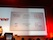
\includegraphics[height=\thumbheight]{free/exactduplicate1.jpg}}
		\doublebox{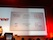
\includegraphics[height=\thumbheight]{free/exactduplicate2.jpg}}
	\end{thumbsequence}
	\begin{thumbsequence}
		
\includegraphics[height=\thumbheight]{free/looseduplicate1.png}
		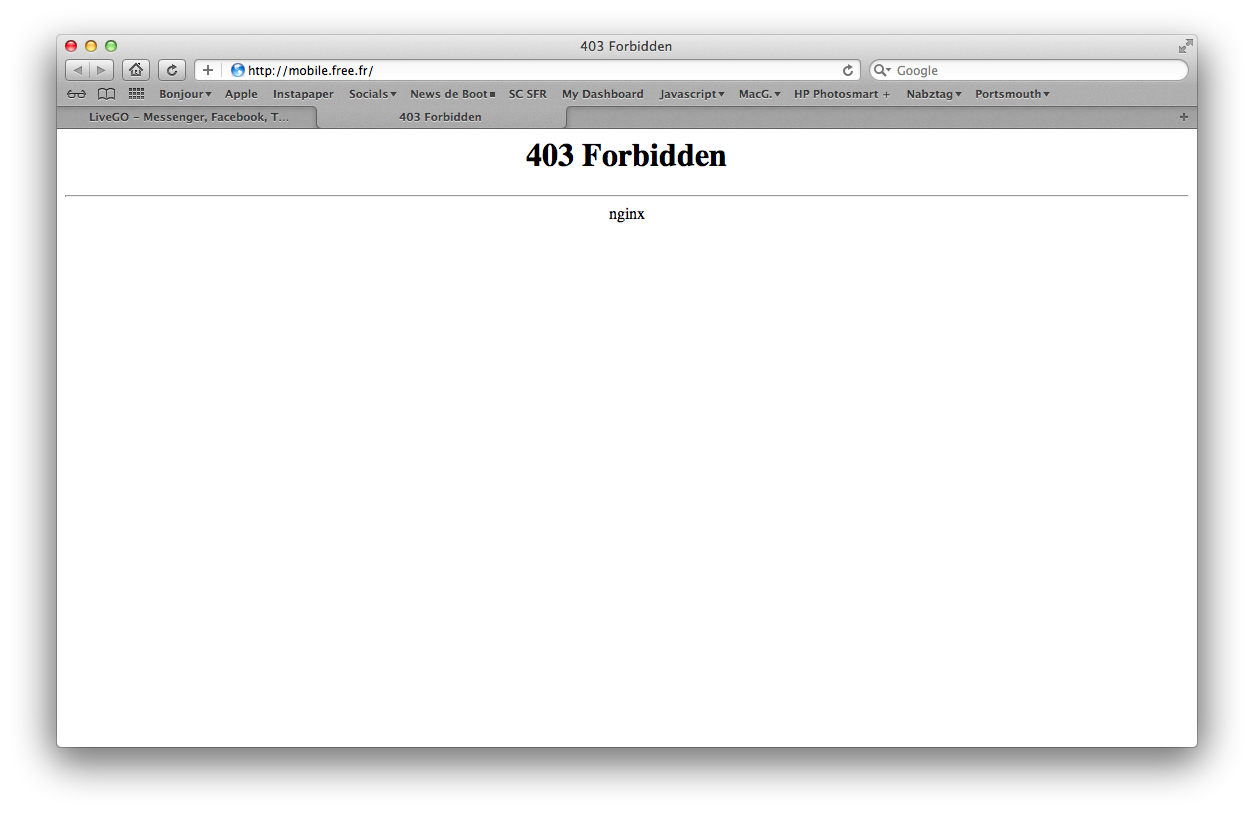
\includegraphics[height=\thumbheight]{free/looseduplicate2.png}
	\end{thumbsequence}
	\begin{thumbsequence}
		
\includegraphics[height=\thumbheight]{free/looseduplicate7.jpg}
		
\includegraphics[height=\thumbheight]{free/looseduplicate8.jpg}
	\end{thumbsequence}
	\\[4pt]
	\begin{thumbsequence}
		
\includegraphics[height=\thumbheight]{free/looseduplicate15.jpg}
		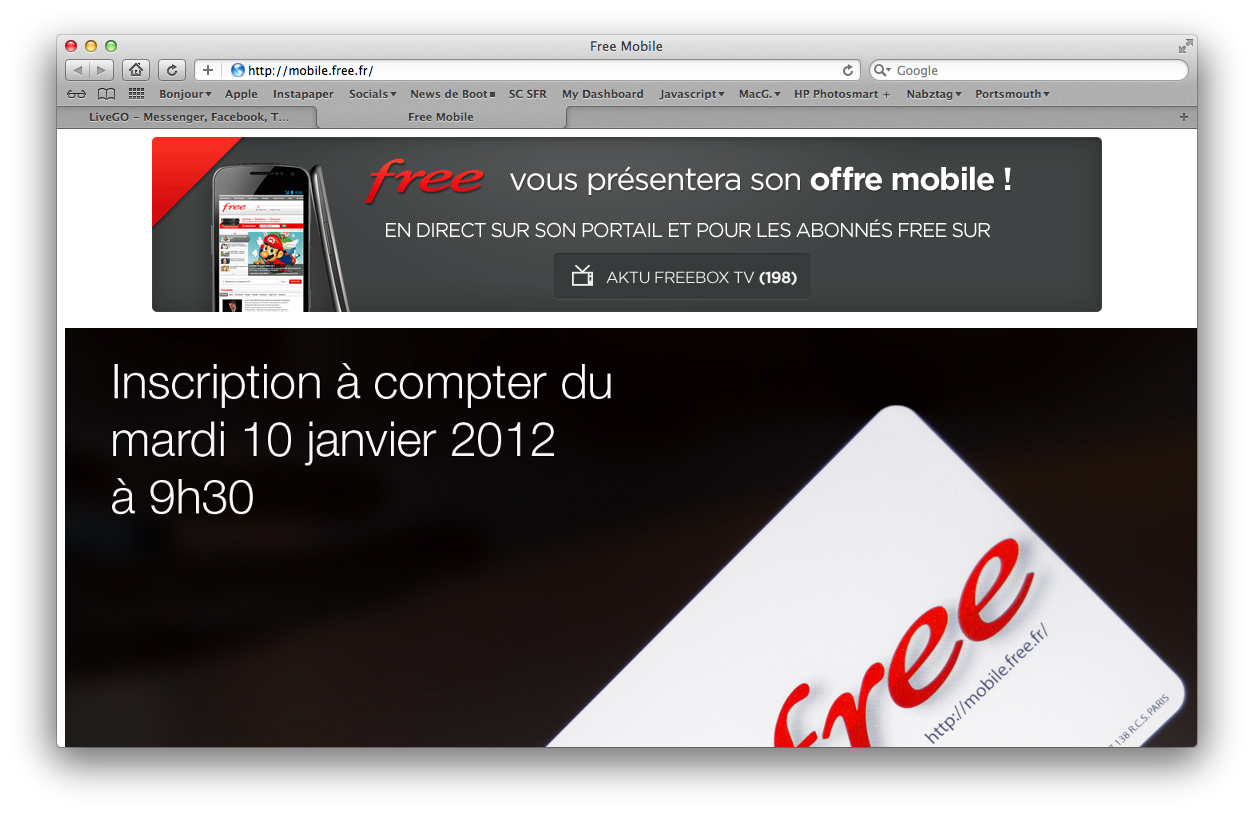
\includegraphics[height=\thumbheight]{free/looseduplicate16.png}
	\end{thumbsequence}
	\begin{thumbsequence}
		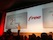
\includegraphics[height=\thumbheight]{free/looseduplicate9.jpg}
		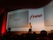
\includegraphics[height=\thumbheight]{free/looseduplicate10.jpg}
		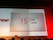
\includegraphics[height=\thumbheight]{free/looseduplicate11.jpg}
	\end{thumbsequence}
	\begin{thumbsequence}
		
\includegraphics[height=\thumbheight]{free/looseduplicate3.jpg}
		
\includegraphics[height=\thumbheight]{free/looseduplicate4.jpg}
	\end{thumbsequence}
	\newstrip
	\begin{thumbsequence}
		
\includegraphics[height=\thumbheight]{free/looseduplicate12.jpg}
		
\includegraphics[height=\thumbheight]{free/looseduplicate13.jpg}
		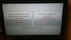
\includegraphics[height=\thumbheight]{free/looseduplicate14.jpg}
	\end{thumbsequence}
	\begin{thumbsequence}
		
\includegraphics[height=\thumbheight]{free/looseduplicate5.jpg}
		
\includegraphics[height=\thumbheight]{free/looseduplicate6.jpg}
	\end{thumbsequence}
\end{tabular}

\begin{tabular}{p{\textwidth}}
\eventtitle{Costa Concordia Disaster}
	\begin{thumbsequence}
		
\includegraphics[height=\thumbheight]{concordia/looseduplicate1.jpg}
		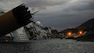
\includegraphics[height=\thumbheight]{concordia/looseduplicate2.jpg}
	\end{thumbsequence}
	\begin{thumbsequence}
		
\includegraphics[height=\thumbheight]{concordia/looseduplicate3.jpg}
		
\includegraphics[height=\thumbheight]{concordia/looseduplicate4.jpg}
	\end{thumbsequence}
	\begin{thumbsequence}
		
\includegraphics[height=\thumbheight]{concordia/looseduplicate5.jpg}
		
\includegraphics[height=\thumbheight]{concordia/looseduplicate6.jpg}
	\end{thumbsequence}
\end{tabular}

\begin{tabular}{p{\textwidth}}
\eventtitle{CES Las Vegas}
	\begin{thumbsequence}
		
\includegraphics[height=\thumbheight]{ces/looseduplicate1.jpg}
		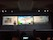
\includegraphics[height=\thumbheight]{ces/looseduplicate2.jpg}
		
\includegraphics[height=\thumbheight]{ces/looseduplicate3.jpg}
		
\includegraphics[height=\thumbheight]{ces/looseduplicate4.jpg}
		
\includegraphics[height=\thumbheight]{ces/looseduplicate5.jpg}
	\end{thumbsequence}
	\begin{thumbsequence}
		
\includegraphics[height=\thumbheight]{ces/looseduplicate6.jpg}
		\includegraphics[height=\thumbheight]{ces/looseduplicate7.jpg}
	\end{thumbsequence}
	\begin{thumbsequence}
		\includegraphics[height=\thumbheight]{ces/looseduplicate8.jpg}
	\end{thumbsequence}
\end{tabular}
\caption[Sample photos for some of the considered nine events]
  {Sample photos for some of the considered nine events
         (showing only exact- or near-duplicate media items)}
\label{fig:sequences}
\end{figure*}


\subsection{The Need for Media Item Deduplication}
\label{sec:the-need-for-media-item-deduplication}

Given our broad approach to retrieve media items
across multiple social networks,
we observed many exact-duplicate or near-duplicate media items.
Oftentimes, these duplicates stem from users who
cross-post to several social networks.
Instead of trying to filter out cross-posted items,
we rather keep them and cluster them.
We are especially interested in social interactions
that media items can trigger.
For example, if one and the same photo
is cross-posted to separate networks,
it can retrieve shares, likes, views, or comments
independently on each of those networks.
By clustering media items, we get a~higher-level view on
a~media item cluster's overall performance on different networks.
We also observed media items that were near-duplicates,
for example, from people who attended the same event like a~concert
and who took photos of the stage from almost the same angle.
Similar to exact-duplicates,
by clustering near-duplicate media items,
we can treat them like exact-duplicates to get the same
network-agnostic viewpoint.
We will examine reasons for exact-duplicate and near-duplicate
media item content and ways to deal with it in \autoref{cha:media-item-deduplication}.

\subsection{The Need for Ranking Media Items}

Our ultimate goal is to generate media galleries
that \emph{visually} and \emph{audially} summarize events.
Especially given high-recall search terms,
we need a~way to rank and prune media items.
Popular media items can be displayed bigger, longer,
or with a~special decoration like a~thicker border
in comparison to less popular media items.
For videos, the audio part poses a~challenge.
In our experiments, we observe that intermixing the audio
of all videos of an event often generates
a very characteristic \emph{noise cloud}
that \emph{audially} conveys the event's atmosphere very well.
A~good example is the Assad Speech event,
where a~mix of Arabic voices blends nicely
with the speech of a~US politician.
A~different example is the CES Las Vegas event,
where the atmosphere of a~big exposition with music,
announcements, and technical analysis becomes alive.
We will have a~closer look at media item ranking in
\autoref{cha:media-item-ranking}.

\section{Conclusions}

In this chapter, we have presented a~generic media extractor
for extracting media items shared on social networks to
illustrate known events.
We have proposed a~common abstraction layer on top of the
social networks' native data formats to align search results.
Our approach to extracting media items and associated
textual microposts covers already most of
the Western world's social networks.
Context-aware multimedia analysis will bring a~new range of
parameters into play since many media items contain a~message
that is complementary to the text.
For example, facial detection~\cite{viola2004facedetection}
and eventually recognition~\cite{wright2009facerecognition}
can signify the presence of specific people in a~media item.
Optical Character Recognition (OCR) can generate
additional textual signals from media items.
As visual recognition systems grow more powerful,
more objects will eventually be recognizable by
machines~\cite{serre2007objectrecognition},
which would allow for generating \emph{visual hashtags}
that describe the content
\emph{inside} of the media item.
Extracted features in all three categories
(\emph{textual}---from the micropost,
\emph{visual}---from the media item,
and \emph{social}---from the social network
in the form of social interactions)
can serve as ranking criteria, be it in isolation
or in combination by introducing a~ranking formula.
As a~result, this will also positively influence
the diversity of automated summarizations.

Nonetheless, it remains important to view the media and the
accompanying microposts as a~whole, since the text
could convey a~sentiment about,
or an explanation of the visual data.
Using named entity recognition as outlined in
\autoref{cha:micropost-annotation},
the important semantic elements in the micropost get identified. 
The content of the message can subsequently be used
to narrow down the search space for visual factors
enabling cross-fertilization between the textual
and visual analysis, which results in effective context-aware analysis possibilities~\cite{verborgh2012multimediaannotation,rizzo2012whatfresh}.
Finally, by leveraging the \emph{LOD} cloud,
we can use that knowledge to get a~more diverse view on events.
At time of writing, the so-called
\emph{Operation Pillar of
Defense\footnote{\url{http://en.wikipedia.org/wiki/Operation_Pillar_of_Defense}, accessed July 15, 2013}}
by the Israeli armed forces
causes ongoing conflicts between Palestinians and Israelis.
Using the LOD cloud, promising search terms like, for example,
\emph{gaza}, can be easily looked up in different languages
like Hebrew or Arabic.
In practice, these additional search terms return interesting
new media items that a~pure monolingual search
would not have revealed---oftentimes,
and especially in the concrete case,
at the expense of neutrality.
We are confident that the additional coverage
from more angles helps sharpen one's own viewpoint of an event,
especially with the option of translating microposts
authored in foreign languages%
---which is supported by our approach---%
as mentioned in \autoref{sec:machine-translation}.

\section*{Chapter Notes}
This chapter is partly based on the following publications:
\todo{Add publications}

\bibliographystyle{plainnat}
\clearpage
\bibliography{backmatter/references}
